\section{Finite element analysis and PiNN}
\subsection{Finite Element Analysis}
\label{sec:metapde-fea}
PDEs are most naturally posed in their \emph{strong forms}:
\begin{align}
\frac{\partial}{\partial t}u(\bm{x}, t) + \mathcal{N}\left[ u(\bm{x}, t)\right] &= 0 &\bm{x} \in \Omega, t \in [0, T], \label{eq:metapde-strongform} \\
u(\bm{x}, t) &= \bar{u} & \bm{x} \in \partial\Omega, t \in [0, T], \label{eq:metapde-bc} \\
u(\bm{x}, 0) &= \bar{u}_0(\bm{x}) &\bm{x} \in \Omega, t=0. \label{eq:metapde-ic} 
\end{align}
The problem is defined on the spatial domain $\Omega \subset \mathbb{R}^{d_\Omega}$ with boundary $\partial \Omega$, and defined on the time horizon $[0, T]$. The unknown function in the PDE $u(\bm{x}, t)$ is a function of the spatial coordinate $\bm{x}$ and time coordinate $t$, $u: \Omega \times [0, T] \to \mathbb{R}^{d_u}$. $\partial / \partial t u(\bm{x}, t) $ is the partial derivative of the unknown function $u$ with respect to the time. $\mathcal{N}\left[ u(\bm{x}, t)\right]: (\Omega \to \mathbb{R}^{d_u}) \to (\Omega \to \mathbb{R}^{d_\mathcal{F}})$ is a linear or nonlinear operator involving $u$ and its partial derivatives with respect to the spatial coordinates.\\
When the unknown function $u$ is time independent (i.e., $d/ dt u = 0$), the PDE problem becomes a Boundary Value Problem. Finite Element Method (FEM) is the common numerical solving method for Boundary Value Problems. In the Experiments section, We will use the Fenics \citep{alnaes2015fenics} implementation of FEM to solve the Boundary Value Problems. The FEM solution will serve as a ground truth and baseline comparison for our proposed meta-PDE solver. The FEM involves rewriting the PDE in their \emph{weak form} (also known as the \emph{variational form}). The recipe for converting PDE to their \emph{weak form} is to multiply the governing equation by a \emph{test function} $v$, and then integrate the multiplied equation over the spacial domain $\Omega$. By requiring the equation to hold for all test functions $v \in \mathcal{V}$ that lives in a suitable infinite-dimensional Sobolev space $H^1(\Omega)$, we have a well-defined problem that uniquely determines $u$. The $u$ that is uniquely determined from satisfying the \emph{weak form} equation simultaneously satisfies the PDE posed in the strong form.
\begin{align}
\int_{\Omega} <\mathcal{F}(u)(\bm{x}), v(\bm{x})> d\bm{x} + \int_{\partial \Omega} <\mathcal{G}(u)(\bm{x}), v(\bm{x})> d \bm{x} &= 0 \quad \forall v \in \mathcal{V} \label{eq:metapde-eakform} \\
\mathcal{V} = \left \lbrace v \in H^1(\Omega): v = 0 \quad \text{on} \partial \Omega \right\rbrace
\end{align}
To solve the variational problem numerically with FEM, we let $\mathcal{V}$ be a class of piecewise low-degree polynomials over the domain, parameterized by some finite number of interpolating points. We fix the values of the interpolating points on the boundary, form a set of basis vectors $v$ for $\mathcal{V}$, rewrite the weak form of the PDE as a linear or nonlinear system representing the set of constraints that must be satisfied, and solve the system with an appropriate linear or nonlinear solver.\\
Figure \ref{fig:metapde-poisson} shows as an example the Poisson problem on a disc. For this simple problem we have $\mathcal{F}(u) = \nabla^2 u - f$, for a spatially varying source term $f$, and $\mathcal{G}(u) = u$, i.e. enforcing $u=0$ on the boundary. 
\begin{figure}[t]
  \centering
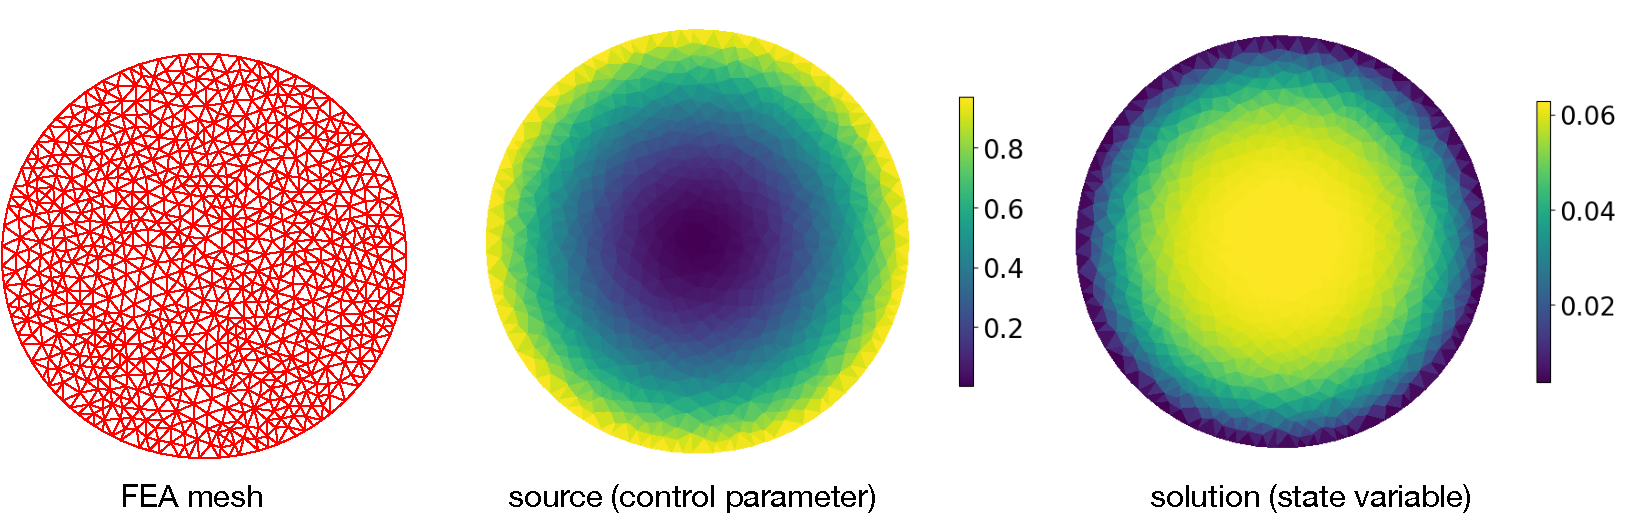
\includegraphics[width=0.8\linewidth]{figures/poisson_equation.pdf}
\caption{Poisson equation on a disc.
Figure: \citet{xue2020amortized}.}%
\label{fig:metapde-poisson}%
\end{figure} \\
When the unknown function $u$ is time dependent (i.e., $du/dt \neq 0$), the PDE problem becomes a Initial Value Problem. One can easily adapt FEM to solve Initial Value Problem by first discretizing the time derivative using a finite difference approximation. At each time step, a Boundary Value Problem is solved independently, and the full solution to the PDE consists of a sequence of time-independent solutions at each time discretization step.\\
We use simple backward finite difference method to approximate the time derivative:
\begin{align}
    \left( \frac{\partial u}{\partial t}\right)^{n+1} \approx \frac{u^{n+1} - u^{n}}{\Delta t} \quad n \in \left \lbrace 0, 1,2,3...N\right\rbrace
\end{align}
The time horizon $[0, T]$ is discretized into a grid of size $N$, with step size $\Delta t = \frac{T}{N}$. Inserting the time discretization into the \emph{strong form} yields:
\begin{align}
    \frac{u^{n+1} - u^{n}}{\Delta t} + \mathcal{N}\left[ u ^{n+1}(\bm{x})\right] &= 0 &\bm{x} \in \Omega, n \in \left \lbrace 0,1,2,3...N\right\rbrace ,  \\
    u^{n+1}(\bm{x}) &= \bar{u} & \bm{x} \in \partial\Omega, n \in \left \lbrace 0,1,2,3...N\right\rbrace , \\
    u^n &= \bar{u}_0(\bm{x}) &\bm{x} \in \Omega, n = 0.
\end{align}
The time discretization step breaks the Initial Value Problem into a sequence of $N$ Boundary Value Problems. At each time step $n$, we solve for $u^{n+1}$ while assuming $u^{n}$ is known from the previous time step. The accuracy of the numerical solution depends on the coarseness of the time grid. 

\subsection{Physics-Informed Neural Networks (PiNN)}
The goal of a PiNN is to its parameters such that it can approximate the solution to the PDE given. In the original proposal, PiNNs can not only incorporate the standard "supervised" data loss, but also a physics-informed loss. The standard supervised loss requires knowing the ground truth solution evaluated at sample points. This "supervised" data loss is useful when experimental data is available. The physics-informed loss consists of the residual of the differential equation. We expect $f_{\theta}$ to satisfy the equations specified above as perfectly as possible. Therefore, one way to incorporate the is to minimize the residual when using $f_\theta$ as the ansatz to the PDE solution $u$. 
\begin{align*}
  \mathcal{J}(u) &= \int_{\Omega} ||\mathcal{N}(u)(\bm{x}, t)||^2_2 dx + \int_{\partial\Omega} ||\mathcal{G}(u)(\bm{x}, t)||_2^2 dx
\end{align*}
During training, we randomly sample collocation points from the PDE domain $\Omega$ and use a set of collocation points $\mathcal{C}$ to approximate the differential equation residual:
\begin{align}
    \mathcal{L}_{\text{PiNN}} = \frac{1}{|\mathcal{C}|} \sum_{(\bm{x}, t) \in \mathcal{C}} || \mathcal{N} (f_{\theta})(\bm{x}, t) ||_2^2  + \frac{1}{|\mathcal{C}|}  \sum_{{(\bm{x}, t) \in \mathcal{\partial \mathcal{C}}} } ||\mathcal{G}(f_{\theta})(\bm{x}, t)||_2^2 
\end{align}
As with \citet{xue2020amortized}, we use this optimization perspective
to derive an efficient training method for our surrogate models.\textcolor{red}{need to complete...}